\documentclass{article}

\usepackage{mmacells}
\usepackage[utf8]{inputenc}
\usepackage{amsmath}
\usepackage{newunicodechar}

\newcommand{\hirayu}{\text{\usefont{U}{min}{m}{n}\symbol{'206}}}

\DeclareFontFamily{U}{min}{}
\DeclareFontShape{U}{min}{m}{n}{<-> udmj30}{}

\usepackage{mmacells}

\usepackage{pandekten}
\usepackage{dashrule}

\usepackage[compat=1.1.0]{tikz-feynman}

%workaround from link
\usetikzlibrary{external}
\immediate\write18{mkdir -p pgf-img}
\tikzexternalize[
  prefix=pgf-img/,
  system call={
    lualatex \tikzexternalcheckshellescape -halt-on-error -interaction=batchmode -jobname="\image" "\texsource" || rm "\image.pdf"
  },
]

\makeatletter
\newcommand*{\shifttext}[1]{%
  \settowidth{\@tempdima}{#1}%
  \hspace{-\@tempdima}#1%
}
\newcommand{\plabel}[1]{%
\shifttext{\textbf{#1}\quad}%
}
\newcommand{\prule}{%
\begin{center}%
\hdashrule[0.5ex]{.99\linewidth}{1pt}{1pt 2.5pt}%
\end{center}%
}

\makeatother

\newcommand{\minusbaseline}{\abovedisplayskip=0pt\abovedisplayshortskip=0pt~\vspace*{-\baselineskip}}%

\setlength{\parindent}{0pt}

\title{Assignment 5}
\author{Ze Chen}

\begin{document}

\maketitle

\plabel{1 (a)}%
The transformation of $U\in \operatorname{U}(n_f)$ is given by $\psi'_j = U_{ji} \psi_j$.
The transformation of the nontrivial element in $\mathbb{Z}_2$ is given by $\psi'_j = \gamma^0 \psi_j$.
The fermion mass term $m\overline{\psi}\psi$ is forbidden.

\plabel{(b--d)}%
The renormalized Lagrangian is given by
\begin{align*}
    \mathcal{L} &= \frac{1}{2} Z_\phi (\partial_\mu \phi)^2 + i Z_\psi \overline{\psi}_j \slashed{\partial} \psi^j - Z_{\hirayu} g \mu^{\epsilon/2} \phi \overline{\psi}_j \psi^j - \frac{1}{4!} Z_4 \lambda \mu^\epsilon \phi^4 \\
    &= \frac{1}{2} (\partial_\mu \phi)^2 + i\overline{\psi}_j \slashed{\partial} \psi^j - g \mu^{\epsilon/2} \phi \overline{\psi}_j \psi^j - \frac{1}{4!} \lambda \mu^{\epsilon} \phi^4 \\
    &\phantom{{}={}} + \frac{1}{2} \delta_{Z,\phi} (\partial_\mu \phi)^2 + i \delta_{Z,\psi} \overline{\psi}_j \slashed{\partial} \psi^j - \delta_g \mu^{\epsilon/2} \phi \overline{\psi}_j \psi^j - \frac{1}{4!} \delta_\lambda \mu^{\epsilon} \phi^4.
\end{align*}
Now we obtain the counter terms.
\begin{itemize}
    \item $\delta_{Z,\phi}$ is obtained by the finiteness of the following.
    \begin{align*}
        \bigO(\epsilon^0) &= \feynmandiagram [layered layout, inline=(p2.base), horizontal=p1 to p2, small] {
            p1[particle=$p$\vphantom{$Mg$}] --[scalar] c1[],
            c1 --[scalar] p2[particle=$p$\vphantom{$Mg$}],
            c1 --[scalar,out=135,in=45,loop,min distance=4em] c1,
        }; + \feynmandiagram [layered layout, inline=(p2.base), horizontal=p1 to p2, small] {
            p1[particle=$p$\vphantom{$Mg$}] --[scalar] c1[dot],
            c2[dot] --[scalar] p2[particle=$p$\vphantom{$Mg$}],
            c1 --[half left, fermion] c2;
            c1 --[half right, anti fermion] c2;
        }; + \feynmandiagram [layered layout, inline=(p2.base), horizontal=p1 to p2, small] {
            p1[particle=$p$\vphantom{$Mg$}] --[scalar] c1[crossed dot],
            c1 --[scalar] p2[particle=$p$\vphantom{$Mg$}],
        }; \\
        &= -\frac{i\lambda}{2} \int \frac{\dd[d]{k}}{(2\pi)^d} \frac{i}{k^2} - n_f (-ig)^2 \int \frac{\dd[d]{k}}{(2\pi)^d} \tr\qty[\frac{i(\slashed{k} + \slashed{p})i(\slashed{k})}{(k+p)^2 k^2}] + i p^2 \delta_{Z,\phi}. \\
        \delta_{Z,\phi} &= -\frac{g^2 n_f}{4\pi^2\epsilon}.
    \end{align*}
    \item $\delta_{Z,\psi}$ is obtained by the finiteness of the following.
    \begin{align*}
        \bigO(\epsilon^0) &= \feynmandiagram [layered layout, inline=(p2.base), horizontal=p1 to p2, small] {
        p1[particle=$p$\vphantom{$Mg$}] --[fermion] c1[dot],
        c2[dot] --[fermion] p2[particle=$p$\vphantom{$Mg$}],
        c1 --[scalar,half left] c2;
        c1 --[fermion] c2,
        }; + \feynmandiagram [layered layout, inline=(p2.base), horizontal=p1 to p2, small] {
            p1[particle=$p$\vphantom{$Mg$}] --[fermion] c1[crossed dot],
            c1 --[fermion] p2[particle=$p$\vphantom{$Mg$}],
        }; \\
        &= (-ig)^2 \int \frac{\dd[d]{k}}{(2\pi)^d}\frac{i(\slashed{k})}{k^2} \frac{i}{(k-p)^2} + i\slashed{p}\delta_{Z,\psi}. \\
        \delta_{Z,\psi} &= -\frac{g^2}{(4\pi)^2 \epsilon}.
    \end{align*}
    \item $\delta_g$ is obtained by the finiteness of the following.
    \begin{align*}
        \bigO(\epsilon^0) &= \feynmandiagram [inline=(p1.base), horizontal=v1 to p1, small] {
            p1[particle=\vphantom{$Mg$}] --[scalar] v1[dot],
            p2[] --[anti fermion] v2[dot],
            p3[] --[fermion] v3[dot],
            v1 --[fermion] v2,
            v1 --[anti fermion] v3,
            v2 --[scalar, quarter right] v3,
        }; + \feynmandiagram [inline=(v.base), horizontal=v to p2, small] {
            p1[particle=\vphantom{$Mg$}] --[anti fermion] v[crossed dot],
            p2 --[scalar] v,
            p3 --[fermion] v,
        }; \\
        &= (-i g)^3 \int \frac{\dd[d]{k}}{(2\pi)^d} \frac{i(\slashed{k})}{k^2} \frac{i(\slashed{k})}{k^2} \frac{i}{(k-p)^2}  -i\delta_g. \\
        \delta_g &= \frac{g^3}{8\pi^2 \epsilon}.
    \end{align*}
    \item $\delta_\lambda$ is obtained by the finiteness of the following.
    \begin{align*}
        \bigO(1) &= 3 \times \feynmandiagram [inline=(c2.base), horizontal=c1 to c2, small] {
            p1[particle=\vphantom{$Mg$}] --[scalar] c1[dot],
            p2[particle=\vphantom{$Mg$}] --[scalar] c1,
            c2[dot] --[scalar] p3,
            c2 -- [scalar]p4,
            c1 --[scalar, half left] c2;
            c1 --[scalar, half right] c2;
        }; + 6\times \feynmandiagram [inline=($0.5*(c2.base)+0.5*(c4.base)$), horizontal=c1 to c2, small] {
            c1 --[scalar] p1,
            c2 --[scalar] p2,
            c3 --[scalar] p3,
            c4 --[scalar] p4,
            p1 --[fermion, quarter right] p2,
            p2 --[fermion, quarter right] p3,
            p3 --[fermion, quarter right] p4,
            p4 --[fermion, quarter right] p1,
        }; + \feynmandiagram [inline=(v.base), horizontal=p1 to p3, small] {
            p1 --[scalar] v[crossed dot],
            p2 --[scalar] v,
            p3 --[scalar] v,
            p4 --[scalar] v,
        }; \\
        &= 3\times \frac{(-i\lambda)^2}{2} \int \frac{\dd[d]{k}}{(2\pi)^d} \qty(\frac{i}{k^2})^2 + 6\times (-1) n_f g^4 \int \frac{\dd[d]{k}}{(2\pi)^d} \tr\qty[\qty(\frac{i(\slashed{k})}{k^2})^4] -i\delta_\lambda. \\
        %&= 3\times \frac{i\lambda^2}{(4\pi)^2}\frac{1}{\epsilon} - 6\times \frac{8ig^4}{(4\pi)^2}\frac{1}{\epsilon} - i\delta_\lambda. \\
        \delta_\lambda &= \frac{3\lambda^2 - 48 n_f g^4}{(4\pi)^2}\frac{1}{\epsilon}.
    \end{align*}
\end{itemize}
The bare couplings are given by
\begin{align*}
    \lambda_0 &= \mu^\epsilon Z^{-2}_\phi (\lambda + \delta_\lambda), \\
    g_0 &= \mu^{\epsilon/2} Z^{-1/2}_\phi Z^{-1}_\psi (g + \delta g).
\end{align*}

\plabel{(c)}%
With $\partial \lambda_0/\partial \ln \mu = 0$ and $\partial g_0/\partial \ln \mu = 0$ we obtain
\begin{align*}
    \beta_g &= -\frac{1}{2} \epsilon g + \frac{(3+2n_f)g^3}{(4\pi)^2}, \\
    \beta_\lambda &= -\epsilon \lambda + \frac{3\lambda^2 + 8 n_f g^2\lambda - 48n_f g^4}{(4\pi)^2}.
\end{align*}

\plabel{(b)}%
Therefore,
\begin{align*}
    \gamma_\phi &= \frac{1}{2}\mu \pdv{\mu} \ln(1+\delta_{Z,\phi}) = \frac{1}{2}\frac{n_f g^2}{4\pi^2}, \\
    \gamma_\psi &= \frac{1}{2}\mu \pdv{\mu} \ln(1+\delta_{Z,\psi}) = \frac{1}{2}\frac{g^2}{(4\pi)^2}.
\end{align*}

\plabel{(d)}%
We use equation (12.112) and (12.117) (since Yukawa interaction doesn't add to (12.117) at one-loop level) and find
\begin{align*}
    \gamma_{\phi^2} &= \mu \pdv{\mu}\qty(-\delta_{\phi^2} + \delta_{Z,\phi}) = \frac{\lambda}{(4\pi)^2} + \frac{n_f g^2}{4\pi^2}.
\end{align*}

\plabel{(e)}%
See equation (11.79) (or equation (16.2.16) of Weinberg).
\begin{align*}
    V(\phi_{\text{cl}}) &= \frac{\lambda}{4!}\phi_{\text{cl}}^4 + \frac{1}{64\pi^2}\qty(\frac{\lambda \phi_{\text{cl}}^2}{2})^2 \qty{\log\qty[\frac{\lambda\phi_{\text{cl}}^2}{2M^2}]-\frac{3}{2}} - \frac{n_f}{16\pi^2}  \qty(g^2\phi_{\text{cl}}^2)^2 \qty{\log\qty[\frac{g^2 \phi_{\text{cl}}^2}{M^2}]-\frac{3}{2}}.
\end{align*}

\plabel{(f)}%
The Callan-Symanzik equation for the effective potential is given by equation (13.25)
\begin{align*}
    \qty[\mu\pdv{\mu} + \beta_\lambda \pdv{\lambda} + \beta_g \pdv{g} - \gamma_{\phi} \phi_{\text{cl}} \pdv{\phi_{\text{cl}}}] V_{\text{eff}}(\phi_{\text{cl}},\mu,\lambda,g) &= 0.
\end{align*}

\plabel{(g)}%
The fixed points locates at the solution of $\beta_g = 0$ and $\beta_\lambda = 0$, i.e.
\begin{gather*}
    g_*=0,\quad \lambda_*=0; \\
    g_*=0,\quad \lambda_*=\frac{16\pi^2}{3}\epsilon; \\
    g_*=\pm \frac{2\sqrt{2}\pi \sqrt{\epsilon}}{\sqrt{2n_f+3}},\quad \lambda_*=\frac{8 \pi ^2 \left(-2 n_f+\sqrt{4 (n_f+33) n_f+9}+3\right) \epsilon }{6 n_f+9}.
\end{gather*}

\plabel{(h)}%
\begingroup\minusbaseline%
\begin{gather*}
    \gamma_{\phi*} = 0,\quad \gamma_{\phi*} = \frac{n_f\epsilon}{2n_f+3};\quad \Delta_{\phi} = \frac{2-\epsilon}{2} + \gamma_{\phi*}; \\
    \gamma_{\psi*} = 0,\quad \gamma_{\psi*} = \frac{n_f\epsilon}{4(2n_f+3)}; \quad \Delta_{\phi} = \frac{3-\epsilon}{2} + \gamma_{\psi*}; \\
    \gamma_{\phi^2*} = 0,\quad \gamma_{\phi^2_*} = \frac{\epsilon}{3},\\
    \gamma_{\phi^2*} = \frac{\left(10 n_f\pm \sqrt{4 (n_f+33) n_f+9}+3\right) \epsilon }{6 (2 n_f+3)};\quad \Delta_{\phi^2} = 2-\epsilon + \gamma_{\phi^2*};.
\end{gather*}
\endgroup

\prule
\plabel{2 (a)}%
The DoF of $\operatorname{SU}(N)$ is $N^2-1$.
In particular for $N=3$ the DoF is $8$.

\plabel{(b--d)}%  
Define the matrices.
\begin{mmaCell}{Input}
\mmaSub{t}{1}=\mmaFrac{1}{2}(\{\{0,1,0\},\{1,0,0\},\{0,0,0\}\});
\mmaSub{t}{2}=\mmaFrac{1}{2}\{\{0, -\mmaDef{i}, 0\}, \{\mmaDef{i}, 0, 0\}, \{0, 0, 0\}\};
\mmaSub{t}{3}=\mmaFrac{1}{2}\{\{1, 0, 0\}, \{0, -1, 0\}, \{0, 0, 0\}\};
\mmaSub{t}{4}=\mmaFrac{1}{2}\{\{0, 0, 1\}, \{0, 0, 0\}, \{1, 0, 0\}\};
\mmaSub{t}{5}=\mmaFrac{1}{2}\{\{0,0, -\mmaDef{i}\}, \{0, 0, 0\}, \{\mmaDef{i}, 0, 0\}\};
\mmaSub{t}{6}=\mmaFrac{1}{2}\{\{0, 0, 0\}, \{0, 0, 1\}, \{0, 1, 0\}\};
\mmaSub{t}{7}=\mmaFrac{1}{2}\{\{0, 0, 0\}, \{0, 0, -\mmaDef{i}\}, \{0, \mmaDef{i}, 0\}\};
\mmaSub{t}{8}=\mmaFrac{1}{2\mmaSqrt{3}}\{\{1, 0, 0\}, \{0, 1, 0\}, \{0, 0, -2\}\};
\end{mmaCell}

Evaluate and find $C(r)=1/2$.
\begin{mmaCell}[moredefined={cr},morefunctionlocal={i, j}]{Input}
cr=Tr[Table[Tr[\mmaSub{t}{i}.\mmaSub{t}{j}],\{i,1,8\},\{j,1,8\}]]/8
\end{mmaCell}

\begin{mmaCell}{Output}
\mmaFrac{1}{2}
\end{mmaCell}

Verify that $\tr(t^a t^b) = C(r)\delta^{ab}$.
\begin{mmaCell}[morefunctionlocal={i, j},moredefined={cr}]{Input}
Table[Tr[\mmaSub{t}{i}.\mmaSub{t}{j}],\{i,1,8\},\{j,1,8\}] == cr IdentityMatrix[8]
\end{mmaCell}

\begin{mmaCell}{Output}
True
\end{mmaCell}

Evaluate $f^{abc}$.
\begin{mmaCell}[morefunctionlocal={i, j, k},moredefined={cr},morepattern={\#, i_, j_, k_, x_, x}]{Input}
Select[
    Flatten[
        Table[
            \{i,j,k,-\mmaFrac{\mmaDef{i}}{cr}Tr[(\mmaSub{t}{i}.\mmaSub{t}{j}-\mmaSub{t}{j}.\mmaSub{t}{i}).\mmaSub{t}{k}]\},
            \{i,1,8\},\{j,1,8\},\{k,1,8\}
        ],
        2
    ],
    #[[4]]!=0&
]/.\{\{i_,j_,k_,x_\}:>\mmaSub{f}{\mmaPat{i},\mmaPat{j},\mmaPat{k}}==x\}
\end{mmaCell}

\begin{mmaCell}{Output}
\{\mmaSub{f}{1,2,3}=1,\mmaSub{f}{1,3,2}=-1,\mmaSub{f}{1,4,7}=\mmaFrac{1}{2},\mmaSub{f}{1,5,6}=-\mmaFrac{1}{2},\mmaSub{f}{1,6,5}=\mmaFrac{1}{2},
\mmaSub{f}{1,7,4}=-\mmaFrac{1}{2},\mmaSub{f}{2,1,3}=-1,\mmaSub{f}{2,3,1}=1,\mmaSub{f}{2,4,6}=\mmaFrac{1}{2},\mmaSub{f}{2,5,7}=\mmaFrac{1}{2},
\mmaSub{f}{2,6,4}=-\mmaFrac{1}{2},\mmaSub{f}{2,7,5}=-\mmaFrac{1}{2},\mmaSub{f}{3,1,2}=1,\mmaSub{f}{3,2,1}=-1,\mmaSub{f}{3,4,5}=\mmaFrac{1}{2},
\mmaSub{f}{3,5,4}=-\mmaFrac{1}{2},\mmaSub{f}{3,6,7}=-\mmaFrac{1}{2},\mmaSub{f}{3,7,6}=\mmaFrac{1}{2},\mmaSub{f}{4,1,7}=-\mmaFrac{1}{2},
\mmaSub{f}{4,2,6}=-\mmaFrac{1}{2},\mmaSub{f}{4,3,5}=-\mmaFrac{1}{2},\mmaSub{f}{4,5,3}=\mmaFrac{1}{2},\mmaSub{f}{4,5,8}=\mmaFrac{\mmaSqrt{3}}{2},
\mmaSub{f}{4,6,2}=\mmaFrac{1}{2},\mmaSub{f}{4,7,1}=\mmaFrac{1}{2},\mmaSub{f}{4,8,5}=-\mmaFrac{\mmaSqrt{3}}{2},\mmaSub{f}{5,1,6}=\mmaFrac{1}{2},
\mmaSub{f}{5,2,7}=-\mmaFrac{1}{2},\mmaSub{f}{5,3,4}=\mmaFrac{1}{2},\mmaSub{f}{5,4,3}=-\mmaFrac{1}{2},\mmaSub{f}{5,4,8}=-\mmaFrac{\mmaSqrt{3}}{2},
\mmaSub{f}{5,6,1}=-\mmaFrac{1}{2},\mmaSub{f}{5,7,2}=\mmaFrac{1}{2},\mmaSub{f}{5,8,4}=\mmaFrac{\mmaSqrt{3}}{2},\mmaSub{f}{6,1,5}=-\mmaFrac{1}{2},
\mmaSub{f}{6,2,4}=\mmaFrac{1}{2},\mmaSub{f}{6,3,7}=\mmaFrac{1}{2},\mmaSub{f}{6,4,2}=-\mmaFrac{1}{2},\mmaSub{f}{6,5,1}=\mmaFrac{1}{2},
\mmaSub{f}{6,7,3}=-\mmaFrac{1}{2},\mmaSub{f}{6,7,8}=\mmaFrac{\mmaSqrt{3}}{2},\mmaSub{f}{6,8,7}=-\mmaFrac{\mmaSqrt{3}}{2},\mmaSub{f}{7,1,4}=\mmaFrac{1}{2},
\mmaSub{f}{7,2,5}=\mmaFrac{1}{2},\mmaSub{f}{7,3,6}=-\mmaFrac{1}{2},\mmaSub{f}{7,4,1}=-\mmaFrac{1}{2},\mmaSub{f}{7,5,2}=-\mmaFrac{1}{2},
\mmaSub{f}{7,6,3}=\mmaFrac{1}{2},\mmaSub{f}{7,6,8}=-\mmaFrac{\mmaSqrt{3}}{2},\mmaSub{f}{7,8,6}=\mmaFrac{\mmaSqrt{3}}{2},\mmaSub{f}{8,4,5}=\mmaFrac{\mmaSqrt{3}}{2},
\mmaSub{f}{8,5,4}=-\mmaFrac{\mmaSqrt{3}}{2},\mmaSub{f}{8,6,7}=\mmaFrac{\mmaSqrt{3}}{2},\mmaSub{f}{8,7,6}=-\mmaFrac{\mmaSqrt{3}}{2}\}

\end{mmaCell}

Evaluate $C_2(r)$.
\begin{mmaCell}[moredefined={c2r},morefunctionlocal={i}]{Input}
c2r=Sum[\mmaSub{t}{i}.\mmaSub{t}{i},\{i,1,8\}]
\end{mmaCell}

\begin{mmaCell}{Output}
(\mmaFrac{4}{3}	0	0
0	\mmaFrac{4}{3}	0
0	0	\mmaFrac{4}{3})
\end{mmaCell}

Verify that $d(r) C_2(r) = d(G) C(r)$.
\begin{mmaCell}[moredefined={c2r, cr}]{Input}
3 c2r == 8 cr IdentityMatrix[3]
\end{mmaCell}

\begin{mmaCell}{Output}
True
\end{mmaCell}

\prule

\plabel{3 (a)}%
The plot is given below.
\begin{center}
    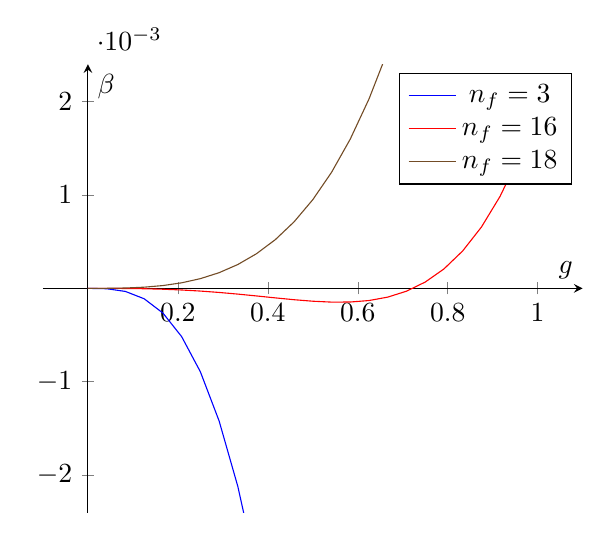
\begin{tikzpicture}
        \begin{axis}[
          ymax=.002, ymin=-.002,
          ylabel=$\beta$,
          xlabel=$g$,
          axis lines=center,
          enlargelimits % maybe you want this as well
        ]
        \addplot+ [mark=none,domain=0:1] {-0.0025665 *\x^5-0.0569932 *\x^3};
        \addplot+ [mark=none,domain=0:1] {0.00403688 *\x^5-0.00211086*\x^3};
        \addplot+ [mark=none,domain=0:1] {0.00505279 *\x^5+0.00633257*\x^3};
        \legend{$n_f=3$,$n_f=16$,$n_f=18$}
        \end{axis}
    \end{tikzpicture}
    \par
    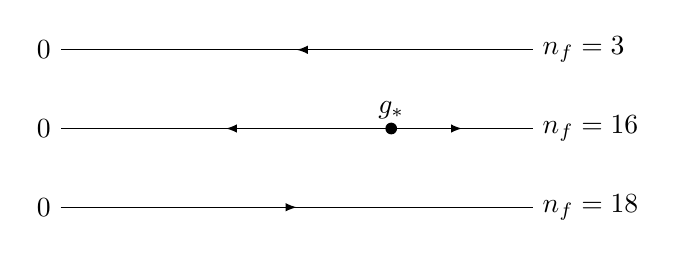
\begin{tikzpicture}[xscale=6]
        \begin{scope}[decoration={
            markings,
            mark=at position 0.5 with {\arrow{latex}}}
            ]
            \draw (0,0) node[left] {$0$};
            \draw (0,1) node[left] {$0$};
            \draw (0,-1) node[left] {$0$};
            \draw (1,0) node[right] {$n_f=16$};
            \draw (1,1) node[right] {$n_f=3$};
            \draw (1,-1) node[right] {$n_f=18$};
            \draw[postaction={decorate}] (1,1)--(0,1);
            \draw[postaction={decorate}] (0.7,0)--(1,0);
            \node at (0.7,0) [circle,fill,inner sep=1.5pt]{};
            \draw (0.7,0) node[above] {$g_*$};
            \draw[postaction={decorate}] (0.7,0)--(0,0);
            \draw[postaction={decorate}] (0,-1)--(1,-1);
        \end{scope}
    \end{tikzpicture}
\end{center}
For $n_f=3$, $g\rightarrow 0$ as $p\rightarrow\infty$, while $g\rightarrow \infty$ as $p\rightarrow 0$.
For $n_f=16$, $g\rightarrow 0$ or $g\rightarrow\infty$ as $p\rightarrow\infty$, while $g\rightarrow g_*$ as $p\rightarrow 0$.
For $n_f=18$, $g\rightarrow \infty$ as $p\rightarrow\infty$, while $g\rightarrow 0$ as $p\rightarrow 0$.

\plabel{(b)}%
$g-g_* \approx A(p/M)^\gamma$ where $g_* = \num{0.723113}$ and $\gamma=\beta'(g_*) = \num{0.00220751}$.

\plabel{(c)}%
It's the anomalous dimension of $\tr(F\wedge F)$. The scaling dimension is $\Delta = d+\gamma$.

\prule

\plabel{4 (a)}%
The vertices are given below.
\begin{align*}
    \feynmandiagram [inline=(v.base), horizontal=p1 to p2, small] {
        p1[particle=${\mu,a}$] --[gluon] v[dot],
        v -- [charged scalar] c2,
        p2[particle=${\nu,b}$] --[gluon] v,
        c1 --[charged scalar] v,
    }; &= i g^2 g^{\mu\nu}(t^a t^b + t^b t^a), \\
    \feynmandiagram [inline=(v.base), horizontal=c1 to c2, small] {
        p1[particle=${\mu,a}$] --[gluon] v[dot],
        v -- [charged scalar] c2[particle=$p_2$],
        c1[particle=$p_1$] --[charged scalar] v,
    }; &= -ig t^a(p_1+p_2)^\mu.
\end{align*}

\plabel{(b)}%
Since the contribution of $\delta_1 - \delta_2 = \delta_1^c - \delta_2^c$ to $\beta$ is universal (independent of the matter field), only the calculation of the matter loop contribution to $\delta_3$ is required.
This is given by
\begin{align*}
    \feynmandiagram [layered layout, inline=(v1.base), horizontal=p1 to p2, small] {
        p1[particle=${\mu,a}$] --[gluon] v1[dot],
        v1 --[charged scalar, half left] v2[dot],
        v2 --[charged scalar, half left] v1,
        v2 --[gluon] p2[particle=${\nu,b}$],
    }; &= \tr((-ig t^b)(-ig t^a))\int \frac{\dd[4]{k}}{(2\pi)^4} \frac{i(2k+q)^\mu i(2k+q)^\nu}{(k+q)^2 k^2} \\
    &= i(q^2 g^{\mu\nu} - q^\mu q^\nu) \delta^{ab} \qty(-\frac{g^2}{(4\pi)^2}\cdot \frac{1}{3} C(r) \cdot \frac{2}{\epsilon} + \cdots).
\end{align*}
Therefore we replace $-4n_f/3$ with $-1/3$ in $\beta$, i.e.
\[ \beta = -\frac{g^3}{(4\pi)^2}\qty[\frac{11}{3}C_2(G) - \frac{1}{3}C(r)]. \]

\end{document}
